\section{Location}
\begin{myremark} Location information is used for positioning, navigation and routing, logistics and location-based services.
\end{myremark}
\begin{mytitle}[Location models] There are two location models: the geometric model based on coordinate systems and the symbolic model based on names.
\end{mytitle}
\begin{center}
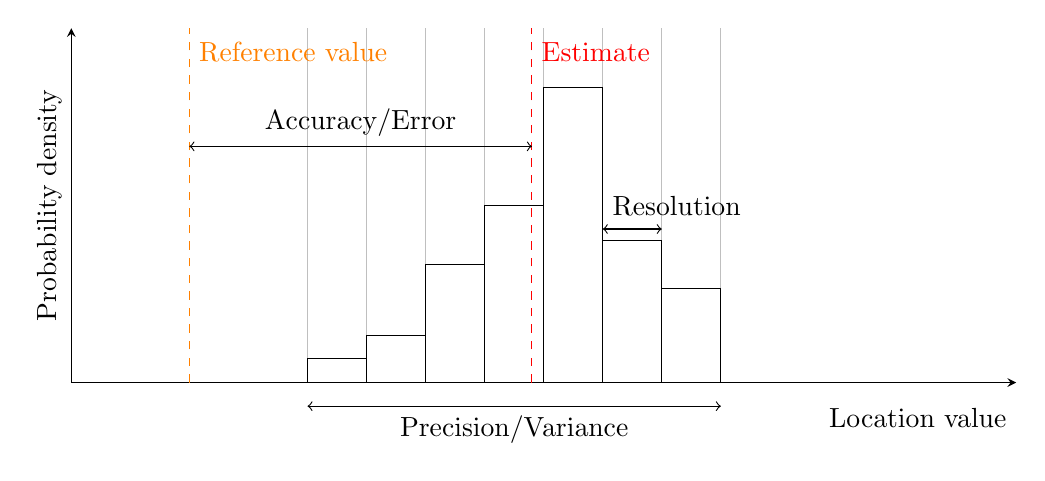
\begin{tikzpicture}

\begin{axis}[
x=1.5cm,
y=1.5cm,
axis y line=left,
axis x line=bottom,
xmax=8,xmin=0,
ymin=0,ymax=3,
xlabel=Location value,
x label style={at={(axis description cs:1,-0.1)},anchor=east},
ylabel=Probability density,
xmajorticks=false,
ymajorticks=false,
width=15cm,
anchor=center,
ybar interval=1,
clip=false
]

\addplot+ [black, fill=white] coordinates {(2,0.2) (2.5,0.4) (3,1) (3.5,1.5) (4,2.5) (4.5,1.2) (5,0.8) (5.5,0.3)};

\draw [dashed, orange] (1,0) -- (1,3);
\node at (1,2.8) [anchor=west, orange] {Reference value};
\draw [dashed, red] (3.9,0) -- (3.9,3);
\node at (3.9,2.8) [anchor=west, red] {Estimate};
\draw [<->, black] (1,2) -- (3.9,2);
\node at (2.45, 2.2) [] {Accuracy/Error};
\draw [<->, black] (4.5, 1.3) -- (5, 1.3);
\node at (4.5, 1.5) [anchor=west] {Resolution};
\draw [<->, black] (2, -0.2) -- (5.5, -0.2);
\node at (3.75, -0.4) [] {Precision/Variance};


\end{axis}
\end{tikzpicture}
\captionof{figure}{Location Terms}
\end{center}
\begin{mytitle}[Characterization of location technologies]\hfill
\begin{itemize}
    \item Tagged (locate a marker) vs. untagged (e.g. vision-based object recognition)
    \item Positioning vs. containment (e.g. check if inside/outside)
    \item Relative positioning vs. absolute positioning
    \item Self-positioning (object knows its position) vs. remote positioning (environment knows objects position)
\end{itemize}
\end{mytitle}

\subsection{Relative and absolute positioning}
\begin{mytitle}[Relative positioning] We can compute the distance from the previous position by the distance itself (odometer), the velocity (speedometer), the acceleration and the height (barometer).
\end{mytitle}
\begin{mytitle}[Absolute Positioning]\hfill
\begin{itemize}
    \item Triangulation: measure the angles to the object from known points at either end of a fixed baseline
    \item Trilateration: measure the distance from the object to three reference points
    \item Multilateration: compare relative distances
\end{itemize}
\end{mytitle}
\begin{mytitle}[Angle of arrival (AOA)] Uses triangulation, used in VHF ominidirectional range (VOR) for aviation and in the global system for mobile communications (GSM) sector.
\end{mytitle}
\begin{mytitle}[Time of arrival (TOA)] Uses trilateration, measures the delay between sending and receiving. When using one-way time synchronization is needed, when using round-trip time no synchronization is needed. Used in global positioning system (GPS) and radar.
\end{mytitle}
\begin{mytitle}[Time difference of arrival (TDOA)] Uses multilateration, three stations compare time difference of signal arrival. Synchronization between stations is required. For the object to learn its own position, the three stations simultaneously emit a signal and the object measures the time difference of their arrival. Because it knows the position of the three reference points, it can learn its own position. Used in mobile phones.
\end{mytitle}

\subsection{Location Systems}
\begin{mytitle}[Global navigation satellite systems (GNSSs)]\hfill
\begin{itemize}
    \item Global positioning system (GPS): US project, 31 satellites total
    \item GLONASS: russian version, 24 satellites total
    \item Beidon/COMPASS: chinese version, 33 satellites total
    \item European galileo system: european version, 22 satellites
\end{itemize}
\end{mytitle}
\begin{mytitle}[Assisted GPS (A-GPS)] A-GPS uses additional data for the GPS receiver through the mobile phone network. This leads to a reduced time to first fix, higher sensitivity for reception of weak satellite signals, reduced power consuption and higher accuracy.
\end{mytitle}
\begin{mytitle}[Positioning via WiFi] Positioning via a database of WiFi access points works particularly in urban areas. It has an accuracy of 15-30 meters.
\end{mytitle}
\begin{mytitle}[Indoor positioning systems] These are all positioning systems with dedicated infrastructures:
\begin{itemize}
    \item Infrared-based systems: these are accurate, have a room-level granularity but are limited by line of sight
    \item RF beacons: these have cell-level granularity
    \item Ultrasound: these include TOA and TDOA, have an accuracy of a few cm but scale poorly
    \item Ultra wide band (UWB): these use four reference stations and have an accuracy of around 20 cm
    \item Others like magnetic and optical systems, these are often targeted at specialized applications
\end{itemize}
\end{mytitle}
\begin{mytitle}[Location APIs] Location APIs contain support for GPS and mobile/wireless network infrastructure location info, support for periodic location updates/proximity alerts, reverse geocoding (coordinates to address) and forward geocoding (address to coordinates).
\end{mytitle}